% GNUPLOT: LaTeX picture with Postscript
\begingroup
  \makeatletter
  \providecommand\color[2][]{%
    \GenericError{(gnuplot) \space\space\space\@spaces}{%
      Package color not loaded in conjunction with
      terminal option `colourtext'%
    }{See the gnuplot documentation for explanation.%
    }{Either use 'blacktext' in gnuplot or load the package
      color.sty in LaTeX.}%
    \renewcommand\color[2][]{}%
  }%
  \providecommand\includegraphics[2][]{%
    \GenericError{(gnuplot) \space\space\space\@spaces}{%
      Package graphicx or graphics not loaded%
    }{See the gnuplot documentation for explanation.%
    }{The gnuplot epslatex terminal needs graphicx.sty or graphics.sty.}%
    \renewcommand\includegraphics[2][]{}%
  }%
  \providecommand\rotatebox[2]{#2}%
  \@ifundefined{ifGPcolor}{%
    \newif\ifGPcolor
    \GPcolortrue
  }{}%
  \@ifundefined{ifGPblacktext}{%
    \newif\ifGPblacktext
    \GPblacktexttrue
  }{}%
  % define a \g@addto@macro without @ in the name:
  \let\gplgaddtomacro\g@addto@macro
  % define empty templates for all commands taking text:
  \gdef\gplbacktext{}%
  \gdef\gplfronttext{}%
  \makeatother
  \ifGPblacktext
    % no textcolor at all
    \def\colorrgb#1{}%
    \def\colorgray#1{}%
  \else
    % gray or color?
    \ifGPcolor
      \def\colorrgb#1{\color[rgb]{#1}}%
      \def\colorgray#1{\color[gray]{#1}}%
      \expandafter\def\csname LTw\endcsname{\color{white}}%
      \expandafter\def\csname LTb\endcsname{\color{black}}%
      \expandafter\def\csname LTa\endcsname{\color{black}}%
      \expandafter\def\csname LT0\endcsname{\color[rgb]{1,0,0}}%
      \expandafter\def\csname LT1\endcsname{\color[rgb]{0,1,0}}%
      \expandafter\def\csname LT2\endcsname{\color[rgb]{0,0,1}}%
      \expandafter\def\csname LT3\endcsname{\color[rgb]{1,0,1}}%
      \expandafter\def\csname LT4\endcsname{\color[rgb]{0,1,1}}%
      \expandafter\def\csname LT5\endcsname{\color[rgb]{1,1,0}}%
      \expandafter\def\csname LT6\endcsname{\color[rgb]{0,0,0}}%
      \expandafter\def\csname LT7\endcsname{\color[rgb]{1,0.3,0}}%
      \expandafter\def\csname LT8\endcsname{\color[rgb]{0.5,0.5,0.5}}%
    \else
      % gray
      \def\colorrgb#1{\color{black}}%
      \def\colorgray#1{\color[gray]{#1}}%
      \expandafter\def\csname LTw\endcsname{\color{white}}%
      \expandafter\def\csname LTb\endcsname{\color{black}}%
      \expandafter\def\csname LTa\endcsname{\color{black}}%
      \expandafter\def\csname LT0\endcsname{\color{black}}%
      \expandafter\def\csname LT1\endcsname{\color{black}}%
      \expandafter\def\csname LT2\endcsname{\color{black}}%
      \expandafter\def\csname LT3\endcsname{\color{black}}%
      \expandafter\def\csname LT4\endcsname{\color{black}}%
      \expandafter\def\csname LT5\endcsname{\color{black}}%
      \expandafter\def\csname LT6\endcsname{\color{black}}%
      \expandafter\def\csname LT7\endcsname{\color{black}}%
      \expandafter\def\csname LT8\endcsname{\color{black}}%
    \fi
  \fi
    \setlength{\unitlength}{0.0500bp}%
    \ifx\gptboxheight\undefined%
      \newlength{\gptboxheight}%
      \newlength{\gptboxwidth}%
      \newsavebox{\gptboxtext}%
    \fi%
    \setlength{\fboxrule}{0.5pt}%
    \setlength{\fboxsep}{1pt}%
    \definecolor{tbcol}{rgb}{1,1,1}%
\begin{picture}(9060.00,9060.00)%
    \gplgaddtomacro\gplbacktext{%
    }%
    \gplgaddtomacro\gplfronttext{%
      \csname LTb\endcsname%%
      \put(444,5102){\makebox(0,0)[r]{\strut{}$-160$}}%
      \csname LTb\endcsname%%
      \put(444,5544){\makebox(0,0)[r]{\strut{}$-120$}}%
      \csname LTb\endcsname%%
      \put(444,5986){\makebox(0,0)[r]{\strut{}$-80$}}%
      \csname LTb\endcsname%%
      \put(444,6428){\makebox(0,0)[r]{\strut{}$-40$}}%
      \csname LTb\endcsname%%
      \put(444,6870){\makebox(0,0)[r]{\strut{}$0$}}%
      \csname LTb\endcsname%%
      \put(444,7312){\makebox(0,0)[r]{\strut{}$40$}}%
      \csname LTb\endcsname%%
      \put(444,7754){\makebox(0,0)[r]{\strut{}$80$}}%
      \csname LTb\endcsname%%
      \put(444,8196){\makebox(0,0)[r]{\strut{}$120$}}%
      \csname LTb\endcsname%%
      \put(444,8638){\makebox(0,0)[r]{\strut{}$160$}}%
      \csname LTb\endcsname%%
      \put(542,4705){\makebox(0,0){\strut{}}}%
      \csname LTb\endcsname%%
      \put(1205,4705){\makebox(0,0){\strut{}}}%
      \csname LTb\endcsname%%
      \put(1868,4705){\makebox(0,0){\strut{}}}%
      \csname LTb\endcsname%%
      \put(2531,4705){\makebox(0,0){\strut{}}}%
      \csname LTb\endcsname%%
      \put(3194,4705){\makebox(0,0){\strut{}}}%
      \csname LTb\endcsname%%
      \put(3857,4705){\makebox(0,0){\strut{}}}%
      \csname LTb\endcsname%%
      \put(4520,4705){\makebox(0,0){\strut{}}}%
      \csname LTb\endcsname%%
      \put(87,6870){\rotatebox{-270.00}{\makebox(0,0){\normalsize $\Psi$}}}%
      \csname LTb\endcsname%%
      \put(2089,7154){\rotatebox{-66.00}{\makebox(0,0){\strut{}\textcolor{black}{\footnotesize 500}}}}%
      \csname LTb\endcsname%%
      \put(2907,6987){\rotatebox{130.00}{\makebox(0,0){\strut{}\textcolor{black}{\footnotesize 400}}}}%
      \csname LTb\endcsname%%
      \put(2146,6682){\rotatebox{-27.00}{\makebox(0,0){\strut{}\textcolor{black}{\footnotesize 400}}}}%
      \csname LTb\endcsname%%
      \put(2313,7650){\rotatebox{154.00}{\makebox(0,0){\strut{}\textcolor{black}{\footnotesize 300}}}}%
      \csname LTb\endcsname%%
      \put(2302,6385){\rotatebox{-39.00}{\makebox(0,0){\strut{}\textcolor{black}{\footnotesize 300}}}}%
      \csname LTb\endcsname%%
      \put(3383,6779){\rotatebox{113.00}{\makebox(0,0){\strut{}\textcolor{black}{\footnotesize 200}}}}%
      \csname LTb\endcsname%%
      \put(1472,8023){\rotatebox{-143.00}{\makebox(0,0){\strut{}\textcolor{black}{\footnotesize 200}}}}%
      \csname LTb\endcsname%%
      \put(2514,6042){\rotatebox{-26.00}{\makebox(0,0){\strut{}\textcolor{black}{\footnotesize 200}}}}%
      \csname LTb\endcsname%%
      \put(1231,8224){\rotatebox{39.00}{\makebox(0,0){\strut{}\textcolor{black}{\footnotesize 100}}}}%
      \csname LTb\endcsname%%
      \put(3216,8239){\rotatebox{42.00}{\makebox(0,0){\strut{}\textcolor{black}{\footnotesize 100}}}}%
      \csname LTb\endcsname%%
      \put(3517,6877){\rotatebox{-71.00}{\makebox(0,0){\strut{}\textcolor{black}{\footnotesize 100}}}}%
      \csname LTb\endcsname%%
      \put(1307,7421){\rotatebox{-43.00}{\makebox(0,0){\strut{}\textcolor{black}{\footnotesize 100}}}}%
      \csname LTb\endcsname%%
      \put(1378,5563){\rotatebox{-33.00}{\makebox(0,0){\strut{}\textcolor{black}{\footnotesize 100}}}}%
      \csname LTb\endcsname%%
      \put(3383,5294){\rotatebox{-28.00}{\makebox(0,0){\strut{}\textcolor{black}{\footnotesize 100}}}}%
      \csname LTb\endcsname%%
      \put(705,7288){\rotatebox{-112.00}{\makebox(0,0){\strut{}\textcolor{black}{\footnotesize 50}}}}%
      \csname LTb\endcsname%%
      \put(3758,7221){\rotatebox{-149.00}{\makebox(0,0){\strut{}\textcolor{black}{\footnotesize 50}}}}%
      \csname LTb\endcsname%%
      \put(2213,8126){\rotatebox{-28.00}{\makebox(0,0){\strut{}\textcolor{black}{\footnotesize 50}}}}%
      \csname LTb\endcsname%%
      \put(2292,5650){\rotatebox{31.00}{\makebox(0,0){\strut{}\textcolor{black}{\footnotesize 50}}}}%
      \csname LTb\endcsname%%
      \put(2531,8982){\makebox(0,0){\strut{}Conformational Energy (meV)}}%
    }%
    \gplgaddtomacro\gplbacktext{%
    }%
    \gplgaddtomacro\gplfronttext{%
      \csname LTb\endcsname%%
      \put(4874,5102){\makebox(0,0)[r]{\strut{}}}%
      \csname LTb\endcsname%%
      \put(4874,5544){\makebox(0,0)[r]{\strut{}}}%
      \csname LTb\endcsname%%
      \put(4874,5986){\makebox(0,0)[r]{\strut{}}}%
      \csname LTb\endcsname%%
      \put(4874,6428){\makebox(0,0)[r]{\strut{}}}%
      \csname LTb\endcsname%%
      \put(4874,6870){\makebox(0,0)[r]{\strut{}}}%
      \csname LTb\endcsname%%
      \put(4874,7312){\makebox(0,0)[r]{\strut{}}}%
      \csname LTb\endcsname%%
      \put(4874,7754){\makebox(0,0)[r]{\strut{}}}%
      \csname LTb\endcsname%%
      \put(4874,8196){\makebox(0,0)[r]{\strut{}}}%
      \csname LTb\endcsname%%
      \put(4874,8638){\makebox(0,0)[r]{\strut{}}}%
      \csname LTb\endcsname%%
      \put(4971,4705){\makebox(0,0){\strut{}}}%
      \csname LTb\endcsname%%
      \put(5634,4705){\makebox(0,0){\strut{}}}%
      \csname LTb\endcsname%%
      \put(6297,4705){\makebox(0,0){\strut{}}}%
      \csname LTb\endcsname%%
      \put(6960,4705){\makebox(0,0){\strut{}}}%
      \csname LTb\endcsname%%
      \put(7623,4705){\makebox(0,0){\strut{}}}%
      \csname LTb\endcsname%%
      \put(8286,4705){\makebox(0,0){\strut{}}}%
      \csname LTb\endcsname%%
      \put(8949,4705){\makebox(0,0){\strut{}}}%
      \csname LTb\endcsname%%
      \put(5031,7851){\rotatebox{37.00}{\makebox(0,0){\strut{}\textcolor{black}{\footnotesize 3.0}}}}%
      \csname LTb\endcsname%%
      \put(8832,6500){\rotatebox{156.00}{\makebox(0,0){\strut{}\textcolor{black}{\footnotesize 3.0}}}}%
      \csname LTb\endcsname%%
      \put(6547,7260){\rotatebox{-78.00}{\makebox(0,0){\strut{}\textcolor{black}{\footnotesize 2.5}}}}%
      \csname LTb\endcsname%%
      \put(5651,8271){\rotatebox{-7.00}{\makebox(0,0){\strut{}\textcolor{black}{\footnotesize 2.5}}}}%
      \csname LTb\endcsname%%
      \put(5409,6940){\rotatebox{-127.00}{\makebox(0,0){\strut{}\textcolor{black}{\footnotesize 2.5}}}}%
      \csname LTb\endcsname%%
      \put(8618,7519){\rotatebox{-88.00}{\makebox(0,0){\strut{}\textcolor{black}{\footnotesize 2.5}}}}%
      \csname LTb\endcsname%%
      \put(8083,6140){\rotatebox{-101.00}{\makebox(0,0){\strut{}\textcolor{black}{\footnotesize 2.5}}}}%
      \csname LTb\endcsname%%
      \put(5500,6320){\rotatebox{91.00}{\makebox(0,0){\strut{}\textcolor{black}{\footnotesize 2.0}}}}%
      \csname LTb\endcsname%%
      \put(6314,7040){\rotatebox{-47.00}{\makebox(0,0){\strut{}\textcolor{black}{\footnotesize 2.0}}}}%
      \csname LTb\endcsname%%
      \put(7233,6000){\rotatebox{-38.00}{\makebox(0,0){\strut{}\textcolor{black}{\footnotesize 2.0}}}}%
      \csname LTb\endcsname%%
      \put(6531,7999){\rotatebox{-101.00}{\makebox(0,0){\strut{}\textcolor{black}{\footnotesize 2.0}}}}%
      \csname LTb\endcsname%%
      \put(7425,6960){\rotatebox{-59.00}{\makebox(0,0){\strut{}\textcolor{black}{\footnotesize 2.0}}}}%
      \csname LTb\endcsname%%
      \put(8359,7080){\rotatebox{64.00}{\makebox(0,0){\strut{}\textcolor{black}{\footnotesize 2.0}}}}%
      \csname LTb\endcsname%%
      \put(5471,5690){\rotatebox{52.00}{\makebox(0,0){\strut{}\textcolor{black}{\footnotesize 1.5}}}}%
      \csname LTb\endcsname%%
      \put(6291,6706){\rotatebox{-17.00}{\makebox(0,0){\strut{}\textcolor{black}{\footnotesize 1.5}}}}%
      \csname LTb\endcsname%%
      \put(6870,5426){\rotatebox{-106.00}{\makebox(0,0){\strut{}\textcolor{black}{\footnotesize 1.5}}}}%
      \csname LTb\endcsname%%
      \put(7650,8582){\rotatebox{-176.00}{\makebox(0,0){\strut{}\textcolor{black}{\footnotesize 1.5}}}}%
      \csname LTb\endcsname%%
      \put(7238,7519){\rotatebox{-45.00}{\makebox(0,0){\strut{}\textcolor{black}{\footnotesize 1.5}}}}%
      \csname LTb\endcsname%%
      \put(8205,7420){\rotatebox{78.00}{\makebox(0,0){\strut{}\textcolor{black}{\footnotesize 1.5}}}}%
      \csname LTb\endcsname%%
      \put(5771,5854){\rotatebox{56.00}{\makebox(0,0){\strut{}\textcolor{black}{\footnotesize 1.0}}}}%
      \csname LTb\endcsname%%
      \put(6570,5482){\rotatebox{-124.00}{\makebox(0,0){\strut{}\textcolor{black}{\footnotesize 1.0}}}}%
      \csname LTb\endcsname%%
      \put(7490,8350){\rotatebox{-162.00}{\makebox(0,0){\strut{}\textcolor{black}{\footnotesize 1.0}}}}%
      \csname LTb\endcsname%%
      \put(8062,7739){\rotatebox{60.00}{\makebox(0,0){\strut{}\textcolor{black}{\footnotesize 1.0}}}}%
      \csname LTb\endcsname%%
      \put(5883,5721){\rotatebox{-132.00}{\makebox(0,0){\strut{}\textcolor{black}{\footnotesize 0.5}}}}%
      \csname LTb\endcsname%%
      \put(7669,8179){\rotatebox{-140.00}{\makebox(0,0){\strut{}\textcolor{black}{\footnotesize 0.5}}}}%
      \csname LTb\endcsname%%
      \put(6960,8982){\makebox(0,0){Dipole Strength (Debye)}}%
    }%
    \gplgaddtomacro\gplbacktext{%
    }%
    \gplgaddtomacro\gplfronttext{%
      \csname LTb\endcsname%%
      \put(444,763){\makebox(0,0)[r]{\strut{}$-160$}}%
      \csname LTb\endcsname%%
      \put(444,1205){\makebox(0,0)[r]{\strut{}$-120$}}%
      \csname LTb\endcsname%%
      \put(444,1647){\makebox(0,0)[r]{\strut{}$-80$}}%
      \csname LTb\endcsname%%
      \put(444,2089){\makebox(0,0)[r]{\strut{}$-40$}}%
      \csname LTb\endcsname%%
      \put(444,2531){\makebox(0,0)[r]{\strut{}$0$}}%
      \csname LTb\endcsname%%
      \put(444,2973){\makebox(0,0)[r]{\strut{}$40$}}%
      \csname LTb\endcsname%%
      \put(444,3415){\makebox(0,0)[r]{\strut{}$80$}}%
      \csname LTb\endcsname%%
      \put(444,3857){\makebox(0,0)[r]{\strut{}$120$}}%
      \csname LTb\endcsname%%
      \put(444,4298){\makebox(0,0)[r]{\strut{}$160$}}%
      \csname LTb\endcsname%%
      \put(542,366){\makebox(0,0){\strut{}$-180$}}%
      \csname LTb\endcsname%%
      \put(1205,366){\makebox(0,0){\strut{}$-120$}}%
      \csname LTb\endcsname%%
      \put(1868,366){\makebox(0,0){\strut{}$-60$}}%
      \csname LTb\endcsname%%
      \put(2531,366){\makebox(0,0){\strut{}$0$}}%
      \csname LTb\endcsname%%
      \put(3194,366){\makebox(0,0){\strut{}$60$}}%
      \csname LTb\endcsname%%
      \put(3857,366){\makebox(0,0){\strut{}$120$}}%
      \csname LTb\endcsname%%
      \put(4519,366){\makebox(0,0){\strut{}$180$}}%
      \csname LTb\endcsname%%
      \put(87,2531){\rotatebox{-270.00}{\makebox(0,0){\normalsize $\Psi$}}}%
      \csname LTb\endcsname%%
      \put(2531,102){\makebox(0,0){\normalsize $\Phi$}}%
      \csname LTb\endcsname%%
      \put(2390,2781){\rotatebox{150.00}{\makebox(0,0){\strut{}\textcolor{black}{\footnotesize 1.3}}}}%
      \csname LTb\endcsname%%
      \put(2270,2355){\rotatebox{-57.00}{\makebox(0,0){\strut{}\textcolor{black}{\footnotesize 1.4}}}}%
      \csname LTb\endcsname%%
      \put(2912,2859){\rotatebox{124.00}{\makebox(0,0){\strut{}\textcolor{black}{\footnotesize 1.5}}}}%
      \csname LTb\endcsname%%
      \put(2511,1819){\rotatebox{-36.00}{\makebox(0,0){\strut{}\textcolor{black}{\footnotesize 1.5}}}}%
      \csname LTb\endcsname%%
      \put(2052,3555){\rotatebox{51.00}{\makebox(0,0){\strut{}\textcolor{black}{\footnotesize 1.6}}}}%
      \csname LTb\endcsname%%
      \put(2164,1627){\rotatebox{-79.00}{\makebox(0,0){\strut{}\textcolor{black}{\footnotesize 1.6}}}}%
      \csname LTb\endcsname%%
      \put(3435,2928){\rotatebox{-15.00}{\makebox(0,0){\strut{}\textcolor{black}{\footnotesize 1.6}}}}%
      \csname LTb\endcsname%%
      \put(3530,2028){\rotatebox{40.00}{\makebox(0,0){\strut{}\textcolor{black}{\footnotesize 1.6}}}}%
      \csname LTb\endcsname%%
      \put(1814,1426){\rotatebox{-81.00}{\makebox(0,0){\strut{}\textcolor{black}{\footnotesize 1.7}}}}%
      \csname LTb\endcsname%%
      \put(1753,3676){\rotatebox{49.00}{\makebox(0,0){\strut{}\textcolor{black}{\footnotesize 1.7}}}}%
      \csname LTb\endcsname%%
      \put(3475,3295){\rotatebox{-26.00}{\makebox(0,0){\strut{}\textcolor{black}{\footnotesize 1.7}}}}%
      \csname LTb\endcsname%%
      \put(3592,1667){\rotatebox{55.00}{\makebox(0,0){\strut{}\textcolor{black}{\footnotesize 1.7}}}}%
      \csname LTb\endcsname%%
      \put(2531,4643){\makebox(0,0){VBA EA (eV)}}%
    }%
    \gplgaddtomacro\gplbacktext{%
    }%
    \gplgaddtomacro\gplfronttext{%
      \csname LTb\endcsname%%
      \put(4874,763){\makebox(0,0)[r]{\strut{}}}%
      \csname LTb\endcsname%%
      \put(4874,1205){\makebox(0,0)[r]{\strut{}}}%
      \csname LTb\endcsname%%
      \put(4874,1647){\makebox(0,0)[r]{\strut{}}}%
      \csname LTb\endcsname%%
      \put(4874,2089){\makebox(0,0)[r]{\strut{}}}%
      \csname LTb\endcsname%%
      \put(4874,2531){\makebox(0,0)[r]{\strut{}}}%
      \csname LTb\endcsname%%
      \put(4874,2973){\makebox(0,0)[r]{\strut{}}}%
      \csname LTb\endcsname%%
      \put(4874,3415){\makebox(0,0)[r]{\strut{}}}%
      \csname LTb\endcsname%%
      \put(4874,3857){\makebox(0,0)[r]{\strut{}}}%
      \csname LTb\endcsname%%
      \put(4874,4298){\makebox(0,0)[r]{\strut{}}}%
      \csname LTb\endcsname%%
      \put(4971,366){\makebox(0,0){\strut{}$-180$}}%
      \csname LTb\endcsname%%
      \put(5634,366){\makebox(0,0){\strut{}$-120$}}%
      \csname LTb\endcsname%%
      \put(6297,366){\makebox(0,0){\strut{}$-60$}}%
      \csname LTb\endcsname%%
      \put(6960,366){\makebox(0,0){\strut{}$0$}}%
      \csname LTb\endcsname%%
      \put(7623,366){\makebox(0,0){\strut{}$60$}}%
      \csname LTb\endcsname%%
      \put(8286,366){\makebox(0,0){\strut{}$120$}}%
      \csname LTb\endcsname%%
      \put(8949,366){\makebox(0,0){\strut{}$180$}}%
      \csname LTb\endcsname%%
      \put(6960,102){\makebox(0,0){\normalsize $\Phi$}}%
      \csname LTb\endcsname%%
      \put(7021,2310){\rotatebox{-43.00}{\makebox(0,0){\strut{}\textcolor{black}{\footnotesize 12}}}}%
      \csname LTb\endcsname%%
      \put(7236,2069){\rotatebox{-30.00}{\makebox(0,0){\strut{}\textcolor{black}{\footnotesize 9}}}}%
      \csname LTb\endcsname%%
      \put(5255,3234){\rotatebox{-53.00}{\makebox(0,0){\strut{}\textcolor{black}{\footnotesize 6}}}}%
      \csname LTb\endcsname%%
      \put(7107,2792){\rotatebox{130.00}{\makebox(0,0){\strut{}\textcolor{black}{\footnotesize 6}}}}%
      \csname LTb\endcsname%%
      \put(7422,1854){\rotatebox{-23.00}{\makebox(0,0){\strut{}\textcolor{black}{\footnotesize 6}}}}%
      \csname LTb\endcsname%%
      \put(8467,1607){\rotatebox{-42.00}{\makebox(0,0){\strut{}\textcolor{black}{\footnotesize 6}}}}%
      \csname LTb\endcsname%%
      \put(7686,2189){\rotatebox{113.00}{\makebox(0,0){\strut{}\textcolor{black}{\footnotesize 3}}}}%
      \csname LTb\endcsname%%
      \put(5496,3877){\rotatebox{-170.00}{\makebox(0,0){\strut{}\textcolor{black}{\footnotesize 3}}}}%
      \csname LTb\endcsname%%
      \put(6531,2591){\rotatebox{-35.00}{\makebox(0,0){\strut{}\textcolor{black}{\footnotesize 3}}}}%
      \csname LTb\endcsname%%
      \put(8748,1369){\rotatebox{50.00}{\makebox(0,0){\strut{}\textcolor{black}{\footnotesize 3}}}}%
      \csname LTb\endcsname%%
      \put(5107,1627){\rotatebox{-108.00}{\makebox(0,0){\strut{}\textcolor{black}{\footnotesize 0}}}}%
      \csname LTb\endcsname%%
      \put(8798,2912){\rotatebox{-74.00}{\makebox(0,0){\strut{}\textcolor{black}{\footnotesize 0}}}}%
      \csname LTb\endcsname%%
      \put(6538,3598){\rotatebox{-62.00}{\makebox(0,0){\strut{}\textcolor{black}{\footnotesize 0}}}}%
      \csname LTb\endcsname%%
      \put(8748,2534){\rotatebox{3.00}{\makebox(0,0){\strut{}\textcolor{black}{\footnotesize 0}}}}%
      \csname LTb\endcsname%%
      \put(6568,2390){\rotatebox{-68.00}{\makebox(0,0){\strut{}\textcolor{black}{\footnotesize 0}}}}%
      \csname LTb\endcsname%%
      \put(8788,1198){\rotatebox{47.00}{\makebox(0,0){\strut{}\textcolor{black}{\footnotesize 0}}}}%
      \csname LTb\endcsname%%
      \put(5767,2531){\makebox(0,0){\strut{}\textcolor{black}{\normalsize \textbf{B}}}}%
      \csname LTb\endcsname%%
      \put(8153,2531){\makebox(0,0){\strut{}\textcolor{black}{\normalsize \textbf{B}}}}%
      \csname LTb\endcsname%%
      \put(6483,2133){\makebox(0,0){\strut{}\textcolor{black}{\normalsize \textbf{A}}}}%
      \csname LTb\endcsname%%
      \put(6960,4643){\makebox(0,0){DBA EA (meV)}}%
    }%
    \gplbacktext
    \put(0,0){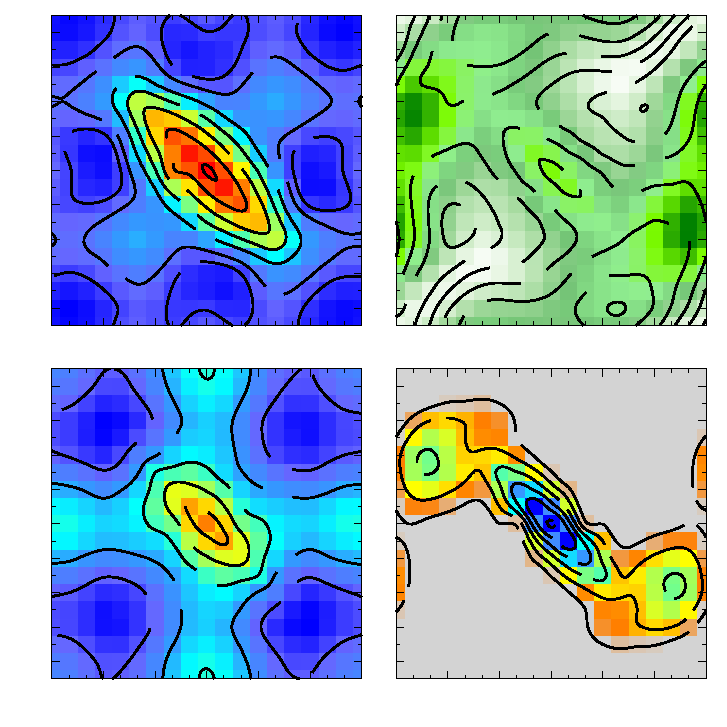
\includegraphics[width={453.00bp},height={453.00bp}]{chapters/results/image/Q0_maps}}%
    \gplfronttext
  \end{picture}%
\endgroup
